\section{Optimal Control of Pitch/Travel without Feedback}\label{sec:prob2}
\label{text:problem2}

\subsection{State space model}
From the model equations in \eqref{eq:model} we get the continuous state space equation
\begin{equation*}
	\begin{bmatrix}
		\dot{\lambda}\\
		\ddot{\lambda}\\
		\dot{p}\\
		\ddot{p}
	\end{bmatrix} = 
	\begin{bmatrix}
		0 & 1 & 0 & 0 \\
		0 & 0 & -K_2 & 0 \\
		0 & 0 & 0 & 1 \\
		0 & 0 & -K_1K_{pp} & -K_1K_{pd}
	\end{bmatrix}
	\begin{bmatrix}
		\lambda	\\
		\dot{\lambda}		\\
		p		\\
		\dot{p}
	\end{bmatrix} +
	\begin{bmatrix}
		0 \\
		0 \\
		0 \\
		K_1K_{pp} \\
	\end{bmatrix}
	p_c
\end{equation*}

or, alternatively
\begin{equation*}
	\begin{bmatrix}
		\dot{\lambda}\\
		\ddot{\lambda}\\
		\dot{p}\\
		\ddot{p}
	\end{bmatrix} = 
	\begin{bmatrix}
		0 & 1 & 0 & 0 \\
		0 & 0 & -0.0663 & 0 \\
		0 & 0 & 0 & 1 \\
		0 & 0 & -5.3095 & -0.9481
	\end{bmatrix}
	\begin{bmatrix}
		\lambda	\\
		\dot{\lambda}		\\
		p		\\
		\dot{p}
	\end{bmatrix} +
	\begin{bmatrix}
		0 \\
		0 \\
		0 \\
		5.3095 \\
	\end{bmatrix}
	p_c
\end{equation*}

However, in an effort to achieve a more accurate model, alternative state space equations are developed from estimated transfer functions based on measured step responses as discussed in \ref{subsection:part1_results}. The model

\begin{equation}
	\begin{bmatrix}
		\dot{\lambda}\\
		\ddot{\lambda}\\
		\dot{p}\\
		\ddot{p}
	\end{bmatrix} = 
	\underbrace{
	\begin{bmatrix}
		0 & 1 & 0 & 0 \\
		0 & -0.03 & -0.39 & 0 \\
		0 & 0 & 0 & 1 \\
		0 & 0 & -7.13 & -3.6
	\end{bmatrix}}_{A_c}
	\begin{bmatrix}
		\lambda	\\
		\dot{\lambda}		\\
		p		\\
		\dot{p}
	\end{bmatrix} +
	\underbrace{
	\begin{bmatrix}
		0 \\
		0 \\
		0 \\
		6.74 \\
	\end{bmatrix}}_{B_c}
	p_c
	\label{eq:sys}
\end{equation}

is constructed from \eqref{eq:p_pc} and \eqref{eq:e_ec}, as well as some preliminary testing. The latter lead to a slight increase in the amount of change in travel rate as a function of pitch.

The reason for the increase in pitch's effect on travel rate is due to the fact that the pitch step response was run with a step size of $20$ degrees. The usual operating range (when aiming for somewhat aggressive maneuvers) is round $30$ to $45$ degrees. This amount of pitch angle will lead to a significant loss of downwards thrust and sequentially elevation. The elevation controller will in turn attempt to compensate by increasing the overall thrust by a large amount, but since the pitch head is far from equilibrium, a substantial amount of that thrust will be affecting the travel rate. This effect overshadows that of the small angle approximation.


\subsection{Discretization}
Let $x = \begin{bmatrix}\lambda&\dot{\lambda}&p&\dot{p}\end{bmatrix}^\top$, $u = p_c$. Using forward Euler with a time step $\Delta t = 0.25$ we are able to obtain an approximate discretization of \eqref{eq:sys}:
\begin{subequations}
\label{eq:dmodel}
\begin{align}
	x_{k+1} &= x_k + \Delta t \dot{x_k} \\
			&= x_k + \Delta t (A_c x_k + B_c u_k)\\
			&= (I + \Delta t A_c) x_k + (\Delta t B_c) u_k \\
			&= A x_k + B u_k
\end{align}
\end{subequations}

where $x_k = x(k\Delta t) \in \mathbb{R}^{n_x}$, $u_k = u(k\Delta t)\in \mathbb{R}^{n_u}$, and
\begin{equation}
	A = 
	\begin{bmatrix}
		1 & 0.25 & 0 & 0 \\
		0 & 0.9925 & -0.0975 & 0 \\
		0 & 0 & 1 & 0.25 \\
		0 & 0 & -1.7825 & 0.1
	\end{bmatrix}, \quad
	B = 
	\begin{bmatrix}
		0 \\
		0 \\
		0 \\
		1.685 \\
	\end{bmatrix}.
\end{equation}

\subsection{Optimal trajectory}

We calculate the trajectory from $x_0 = \begin{bmatrix}\lambda_0&0&0&0\end{bmatrix}^\top$ to $x_f = \begin{bmatrix}\lambda_f&0&0&0\end{bmatrix}^\top$ minimizing the objective function 
\begin{equation}
\label{eq:QC_p}
	\phi = \sum_{i=1}^{N}(\lambda_i - \lambda_f)^2 + rp^2_{c_i}, \quad r \ge 0,
\end{equation}
where we let $\lambda_0 = 0$, $\lambda_f = \pi$.

The parameter $r$ weights the relative importance of low input expendature, in this case set-point for the pitch angle, versus a rapid convergence of the travel trajectory to $\lambda_f$.  Equivalently we can define \eqref{eq:QC_p} in terms of the full state and input variables.

\begin{equation}
	\label{eq:QC_p_QR}
	\phi = \frac{1}{2}\sum_{i=0}^{N-1} (x_{i+1}-x_f)^\top Q (x_{i+1}-x_f) + u_i^\top R u_i,
\end{equation}

where
\begin{equation*}
Q = \begin{bmatrix}1&0&0&0\\0&0&0&0\\0&0&0&0\\0&0&0&0\end{bmatrix}, \quad R = r.
\end{equation*}

The system dynamics \eqref{eq:dmodel} subjects \eqref{eq:QC_p_QR} to the linear equality constraints

\begin{equation}
	\label{eq:eq_constraints}
	\underbrace{
	\left[\begin{array}{cccc | ccccc}
	I	&&&&			-B	&&&			\\
	-A	&\ddots&&&			&\ddots&&	\\
		&\ddots&\ddots&&	&&\ddots&	\\
		&& -A & I&			&&& -B		\\
\end{array}\right]}_{A_{eq} \in \mathbb{R}^{Nn_x \times N(n_x+n_u)}}
\underbrace{
\begin{bmatrix} x_1 \\ \vdots \\ x_N \\ u_0 \\ \vdots \\ u_{N-1} \end{bmatrix}}_{z \in \mathbb{R}^{N(n_x+n_u)\times 1}}
=
\underbrace{
\begin{bmatrix}
-A x_f \\ 0 \\ \vdots \\ 0      
\end{bmatrix}}_{B_{eq}\in \mathbb{R}^{Nn_x \times 1}}.
\end{equation}

To express \eqref{eq:QC_p_QR} in terms of the optimization variable $z$ we define the matrix $G \in \mathbb{R}^{N(n_x+n_u) \times N(n_x + n_u)}$:
\begin{equation*}
	G =
	\begin{bmatrix}
	Q	&&&&&		\\
		&\ddots&&&&	\\
		&&Q&&&		\\
		&&&R&&		\\
		&&&&\ddots&	\\
		&&&&&R		\\
	\end{bmatrix}.
\end{equation*}

With lower and upper bounds imposed on the pitch state and controller set-point, the QP-problem can then be stated:
\begin{subequations}
\label{eq:QP_travel}
\begin{equation}
	\min_z \quad \frac{1}{2} z^\top G z
\end{equation}
	subject to
\begin{align}
	A_{eq} z &= B_{eq}, \\
	p^{\textrm{low}} &\le p_k \le p^{\textrm{high}}, \quad k \in \{1, \dots, N\}.
\end{align}
\end{subequations}

\subsection{Results and discussion}
\eqref{eq:QP_travel} is solved using MATLAB's \texttt{quadprog}. $r = 0.1$ is chosen to achieve a relatively rapid convergence rate in with the effect of maximizing the pitch between the lower and higher bounds. With rapid convergence rate in mind the pitch bounds were set to $\pm\frac{45 \pi}{180}$. The optimal input sequence $u^*$ is applied to the plant in an open loop with results show in figure \ref{fig:opt_openloop}, with the measured trajectory compared to the calculated optimal trajectory $x^*$.

\begin{figure}[hp]
	\centering
		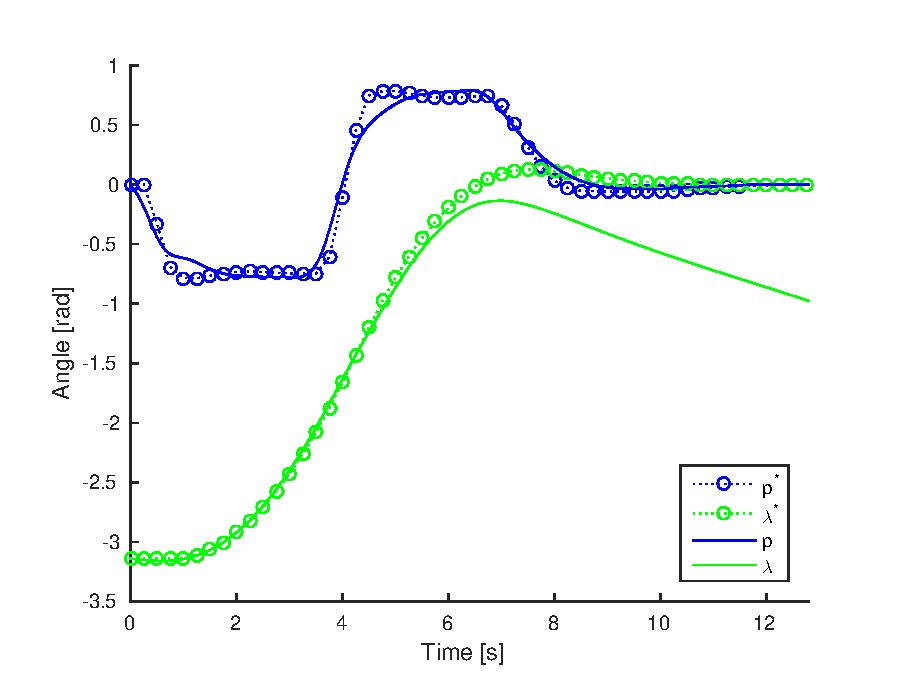
\includegraphics[width=0.85\textwidth]{figures/2/openloop.eps}
	\caption{Optimal vs. measured trajectory and input sequence.}
	\label{fig:opt_openloop}
\end{figure}

The measured trajectory of pitch coincides with the calculated optimal trajectory. The lack of substantial deviation is also a testimonial to the pitch model. Unlike pitch, travel is not controlled by an inner controller, and its deviation from the optimal trajectory should therefore be expected when using open loop.

